
\documentclass[
	%print, % Uncomment to convert colors to CMYK for printing purposes
	%a1papersize, % Uncomment to use an A1 paper size instead of the default A0 paper size
]{ImperialPoster}
\usepackage{helvet}
\usepackage{wrapfig}
\usepackage{placeins}
\usepackage{tcolorbox}

\postertitle{Towards Sustainable Packaging: \\Improving Properties of Biopolymer Films Using Fruit Purées}  % produces ée} % The poster title, can be split across multiple lines manually with \\


% Contributor/author names, can be split across multiple lines manually with \\
% Add affiliations using the \affiliation{} command
\posterauthors{Douglas Penning\affiliation{1}, Alvin Zhu\affiliation{1}, Gabriel Yang\affiliation{1},\\ Manjula Silva\affiliation{1}

\smalltext{\textsuperscript{1}{Department of Materials, Imperial College London}\\}}



%----------------------------------------------------------------------------------------

\begin{document}

\newpage

\titlesection % Output the title section, automatically populated using the information in the POSTER INFORMATION block above

\begin{multicols}{2} % Start the three-column layout

\begin{tcolorbox}[colback=white, colframe=ICLBlue, boxrule=4pt, arc=5pt]
\section{Motivation}

    

    \begin{minipage}{0.55\linewidth}
        \centering
        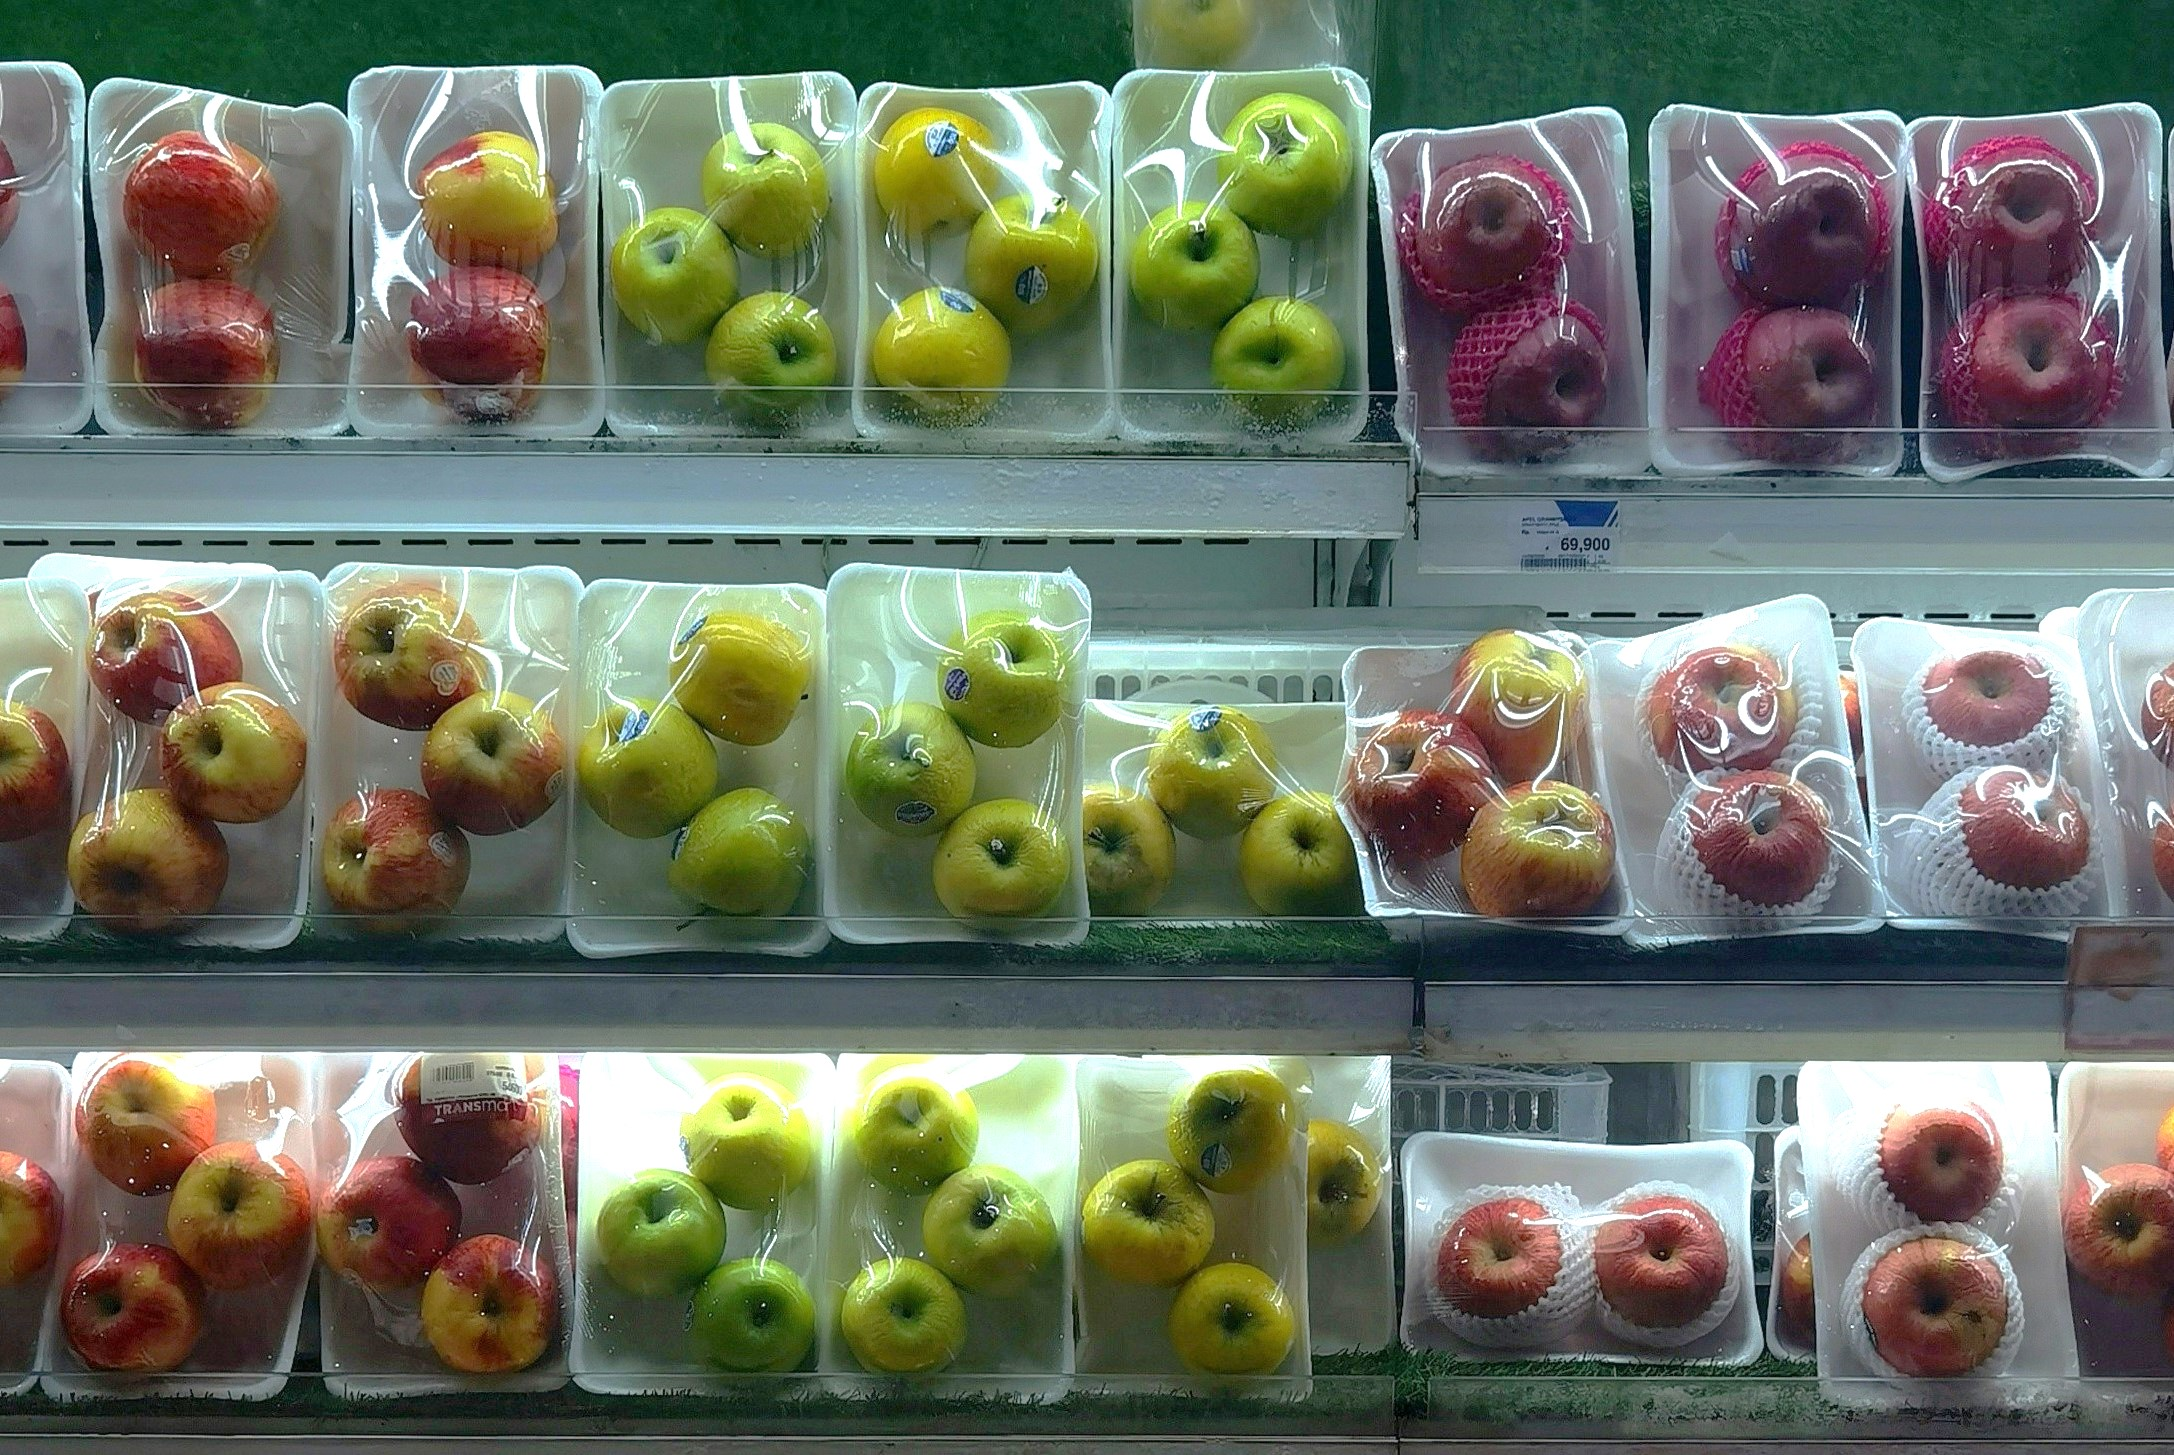
\includegraphics[width=\linewidth]{Package.jpg}
    \end{minipage}%
    \begin{minipage}{0.45\linewidth}
    \centering
    \begin{quote}
    \textcolor{ICLDarkBlue}{
    		23 \% of all Polyethylene film use is for food packaging with $\approx$ 36 kg plastic waste produced per person annually in the EU\textsuperscript{[1]}}
    \end{quote}
    \end{minipage}
    \vspace{0.75em}

    
            Concerns over widespread use of petroleum-based packaging have driven interest in biodegradable starch-gelatine films.
            Transparency of these sustainable alternatives may be improved through the use of papaya\textsuperscript{[2]} and cantaloupe purée additives.
\end{tcolorbox}

\section{Materials \& Methodology}	

    	\begin{figure}[H] % [H] forces the figure to be output where it is defined in the code (it suppresses floating)
        \centering
		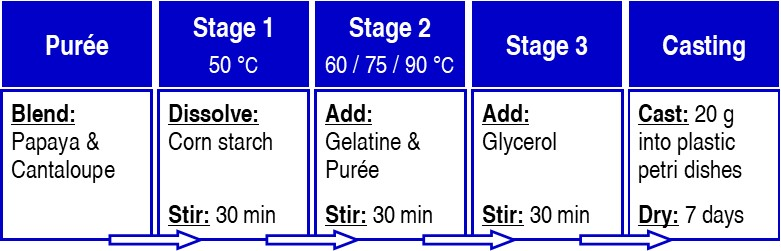
\includegraphics[width = 0.85\linewidth]{Flow.jpg} % Figure image
	\end{figure}	


       
   

        \begin{table}[H] % [H] forces the table to be output where it is defined in the code (it suppresses floating)
        \centering
        \fontsize{0.6\normalbaselineskip}{0.6\normalbaselineskip}\selectfont
		\begin{tabular}{L{0.4\linewidth} C{0.4\linewidth}}
			\toprule
			\textbf{Component} & \textbf{Quantity} \\
			\midrule
		      Corn starch\textsuperscript{2} & 2 wt. \%\\
			Gelatine\textsuperscript{2} &   6 wt. \%\\
		      Papaya\textsuperscript{1} OR Cantaloupe\textsuperscript{1} & 9 - 18 wt. \%\\
            Glycerol\textsuperscript{2} & 6 wt. \%\\
            Deionised Water & q.s. \\
			\bottomrule
		\end{tabular}
	\end{table}
     \smalltext{\textsuperscript{1} Waitrose \& Partners, \textsuperscript{2} Sigma-Aldrich}

	
	\section{Results}
    
    \textcolor{ICLBlue}{Visible light transmittance} ($\lambda$ = 500 nm) was found to \textbf{increase above 13 wt. \% papaya} loadings and appears to be strongly correlated. High papaya loadings reduced particulate count, potentially due to reduced hydrogen bonding between starch-gelatine thus reducing scattering. UV transmittance decreased with addition of either purée.  
    
    \begin{figure}[H] 
    \centering
		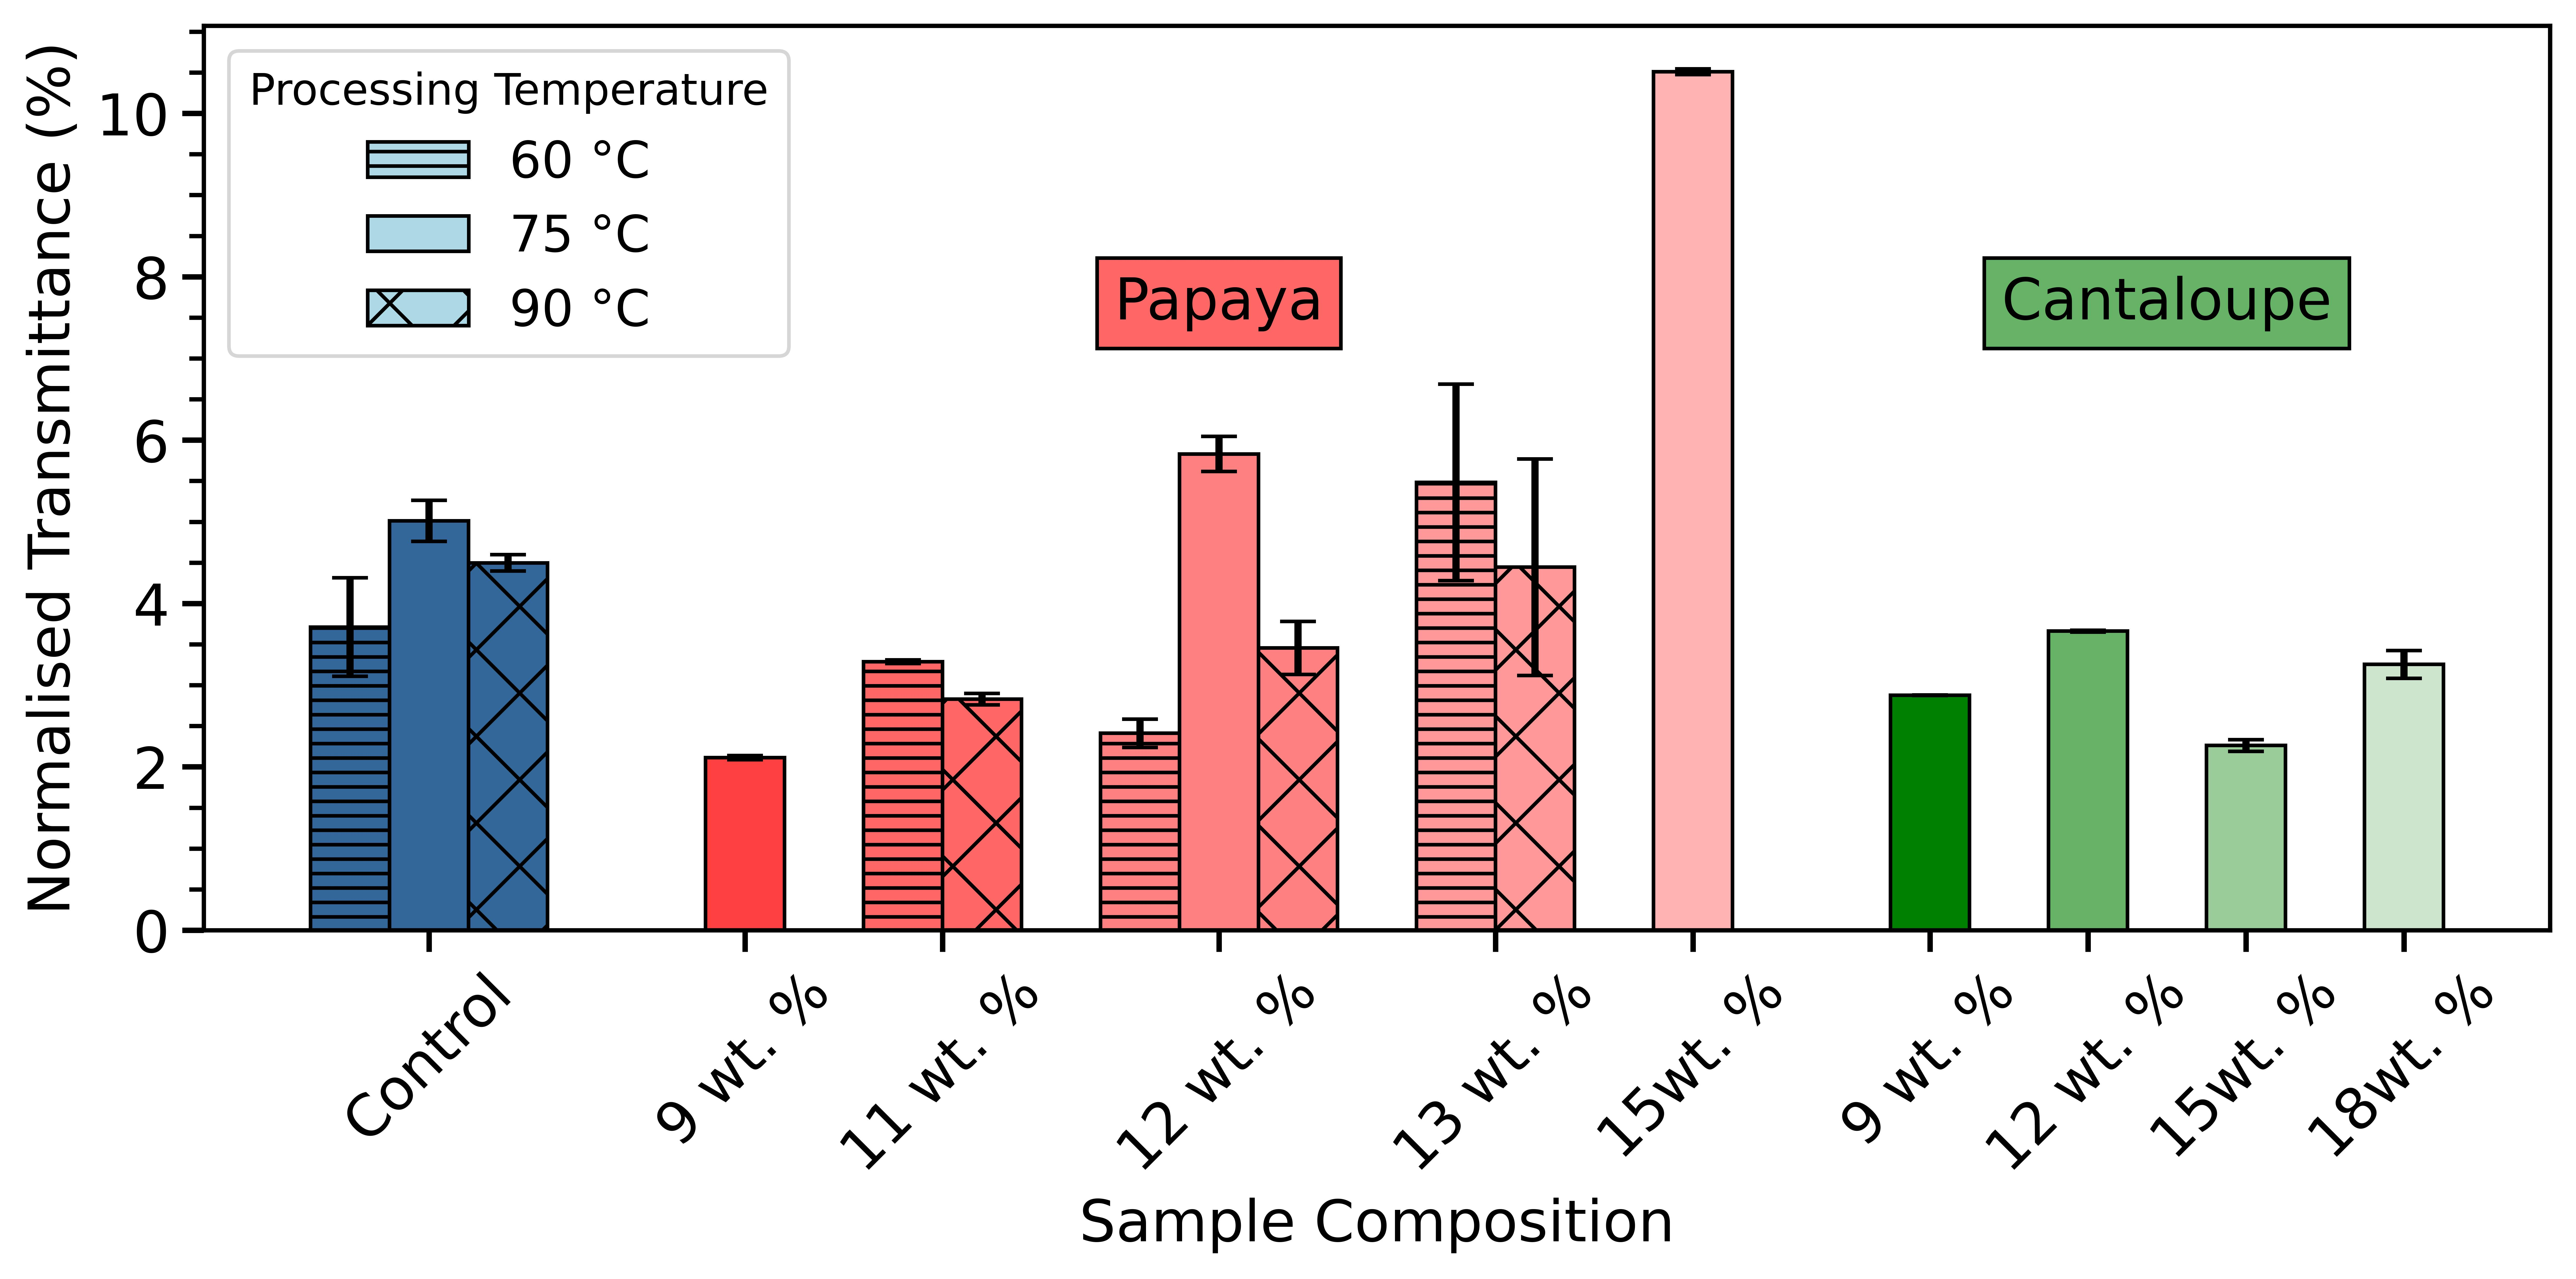
\includegraphics[width=0.98\linewidth]{UVVIS_2C.jpg} % Figure image
		\caption{Normalised average visible light transmittance taken at $\lambda$ = 500 nm using a PerkinElmer Lambda-25. Error bars show standard deviation between repeats.}
	\end{figure}	

	\vspace{-10mm}
	
	
    \textcolor{ICLBlue}{Water contact angle} rose with low papaya content but decreased at higher pur\'{e}e levels. All films were found to \textbf{remain hydrophilic} ($\theta$ < 90°). Sugars disrupt hydrogen bonding and reduce crystallinity thus increasing wettability.

     Rougher air-facing surfaces enhanced hydrophilicity via the Wenzel effect \textsuperscript{[3]}. Higher processing temperature increased hydrophobicity.

    \begin{figure}[H] 
    \centering
    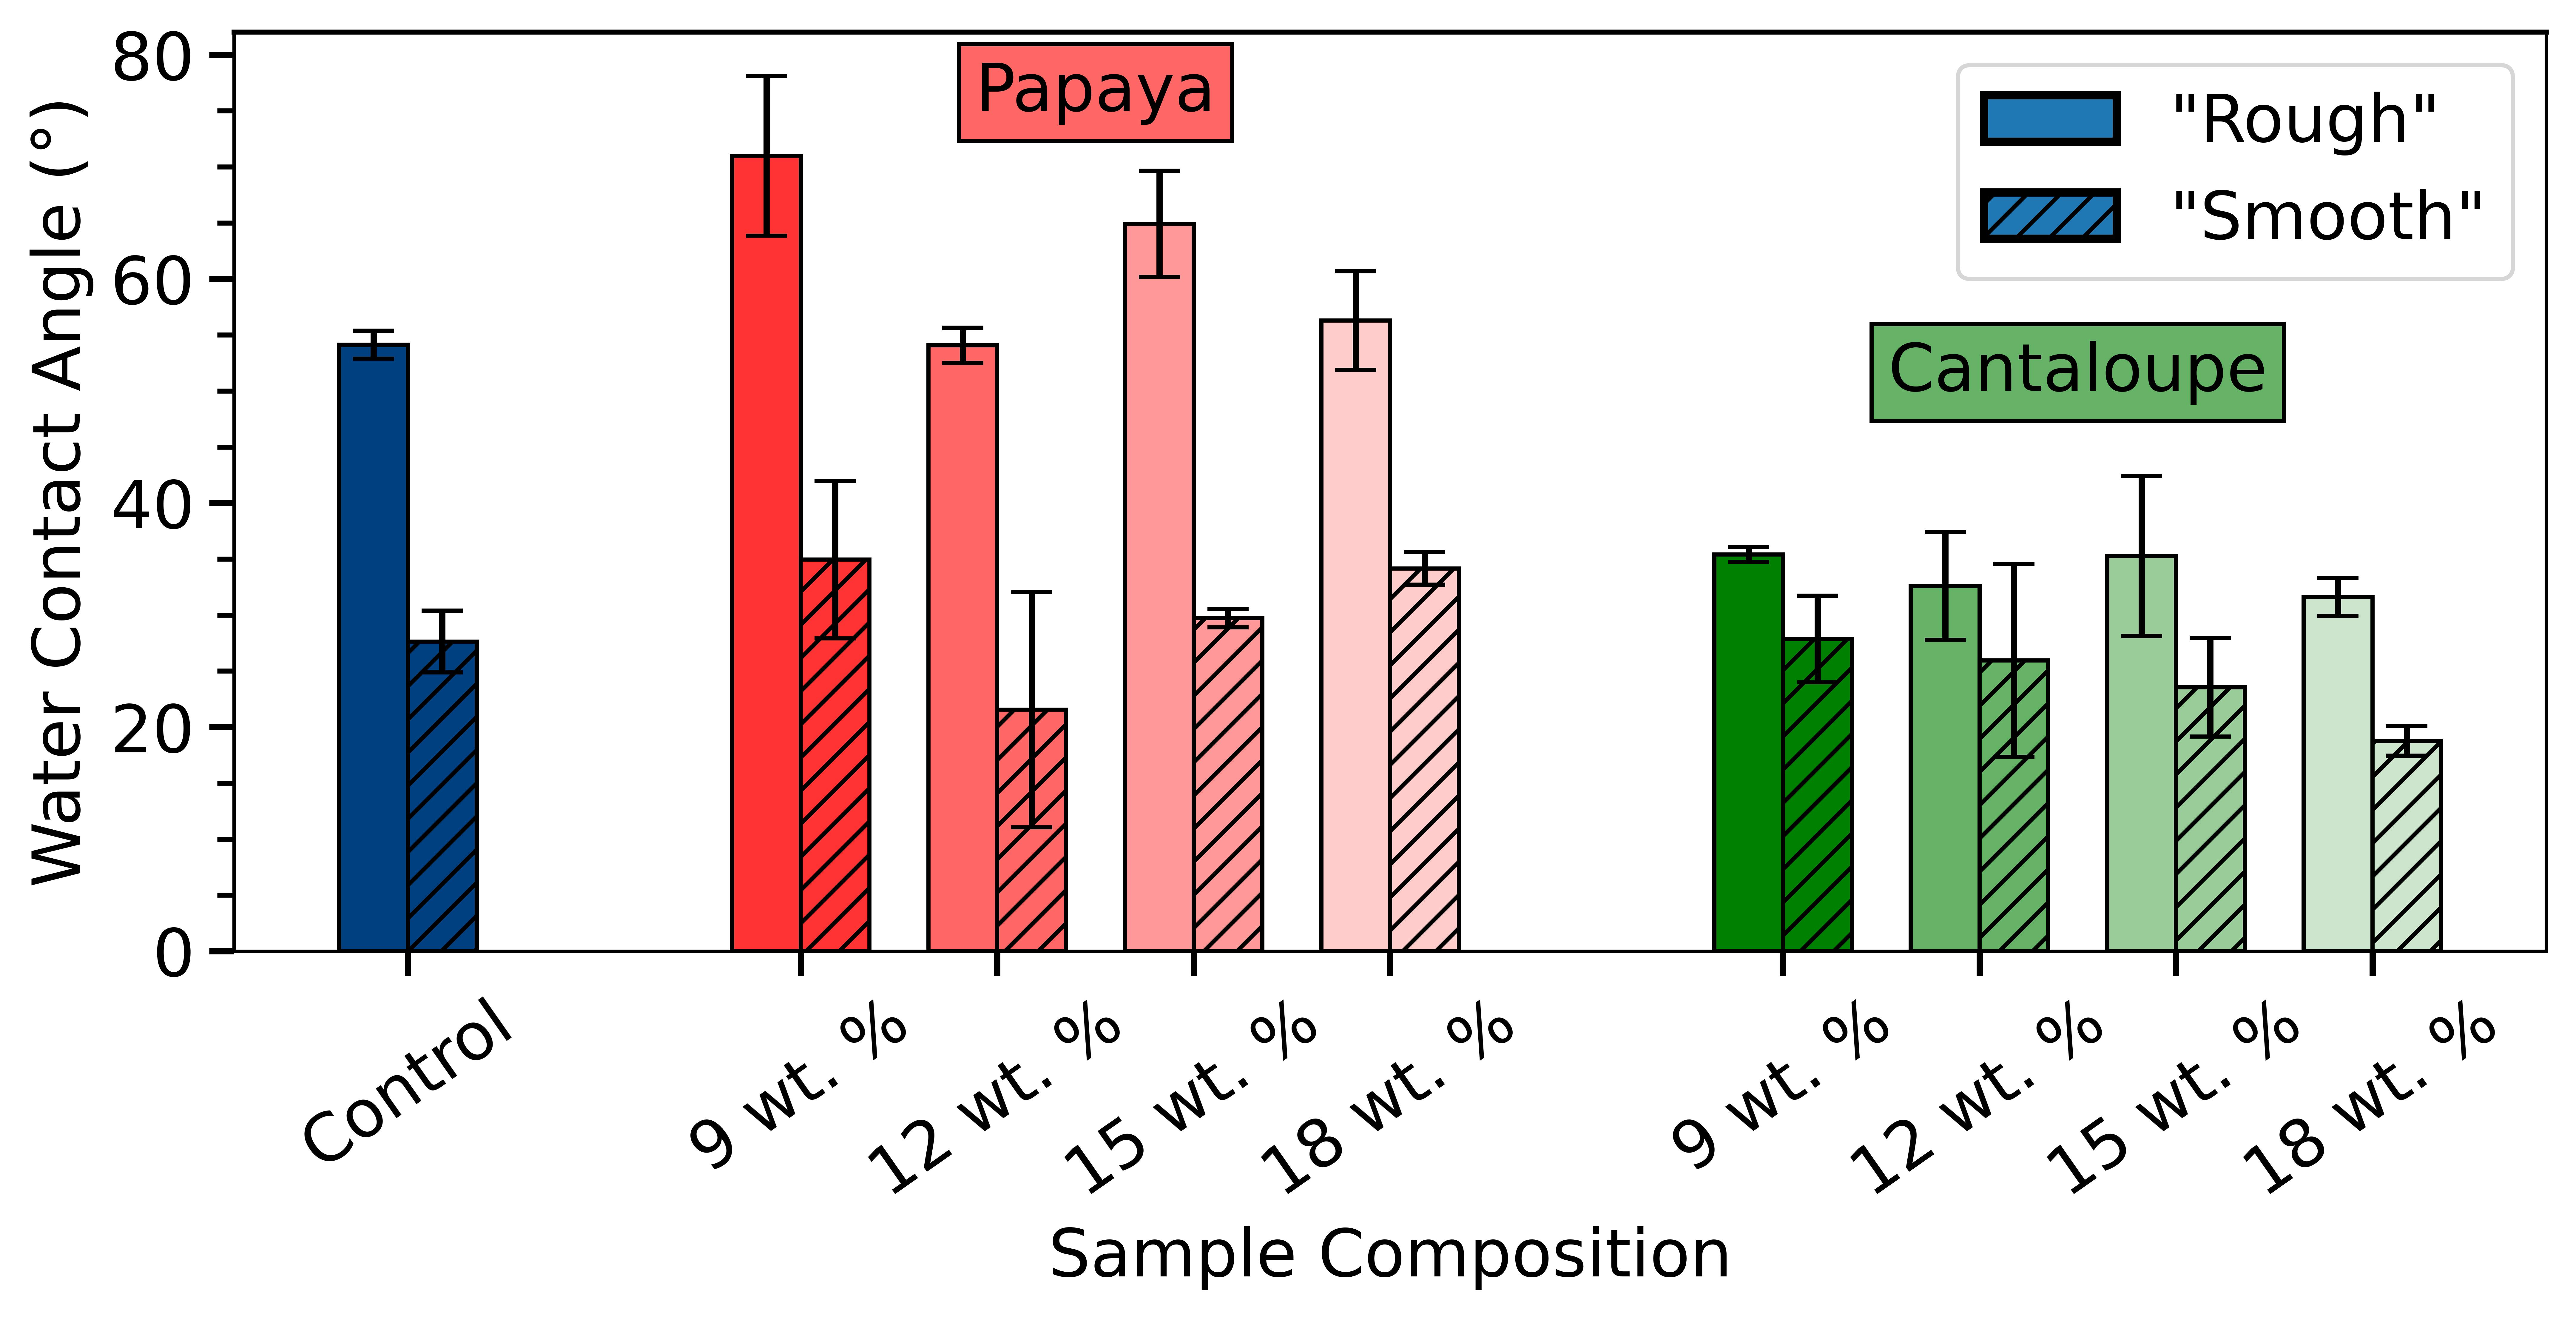
\includegraphics[width=0.95\linewidth]{CA_2C.jpg} % Figure image
    \caption{Water contact angle (°) measured via sessile drop for samples produced at a Stage 2 temperature of 75 $^{\circ}$C (DataPhysics 15EC: resolution = 1°, droplet volume = 5 µL). Error bars represent standard deviation between repeats. Hatched bars show the “smooth” mould facing side of the film.}
    
	\end{figure}

\begin{figure}[H]
    \centering
    \begin{minipage}{0.56\linewidth}
        \centering
        \includegraphics[width=\linewidth]{TS_FINAL.jpg}
    \end{minipage}
    \hfill
    \begin{minipage}{0.38\linewidth}
        \raggedright
        \hyphenpenalty=10000
        \exhyphenpenalty=10000
        \vspace{-45mm}
        Papaya loading significantly reduced \textcolor{ICLBlue}{mechanical performance}, while cantaloupe had minimal impact on elongation at break (\textit{EAB}), and tensile strength (\textit{TS}).

        \vspace{35mm}

        Higher processing temperature notably decreased \textit{EAB} (except Controls), indicating changes to the papaya composition and interactions. 
    \end{minipage}
    \caption{Elongation at break for polymer samples showing mean values with standard deviation error bars. \textbf{(A)} Samples produced at 75\,\textdegree C and \textbf{(B)} papaya samples produced at 60 and 90\,\textdegree C. Measured using ZwickRoell\texttrademark~z010 at test speed of 10\,mm/min.}
\end{figure}



    \begin{tcolorbox}[colback=white, colframe=ICLBlue, boxrule=4pt, arc=5pt]
    \section{Conclusion}
   
	  \begin{itemize}
      \item Light transmittance ($\lambda$ = 500 nm) \textbf{positively correlates} with\\ papaya content; $\approx$ 110\% increase observed using 15 wt. \% papaya
      \item Addition of purée \textbf{reduces UV transmittance}
      \item Papaya pure\'{e} reduces \textit{TS}, \textit{EAB} \& E; low cantaloupe loadings\\ increase modulus and have negligible effect on \textit{EAB}
      \item 60\textdegree C processing temperature found to be optimal for investigated properties
      \item Polymer packaging film application drives property requirements, guiding optimal composition

    \end{itemize}
    \end{tcolorbox}




  
\vspace{1mm}
\textcolor{ICLBlue}{\textbf{Summary:}} Demonstrated a clear improvement in film optical performance, and reduced UV transmittance.\vspace{-0.5em}
\textcolor{ICLBlue}{\rule{\linewidth}{0.2pt}}
\textbf{\textcolor{ICLBlue}{Future research:}} {Refine drying protocols and processing temperature with controlled purée composition.}
  
\vspace{0.5em}
\smalltext{
    \textsuperscript{\textbf{[1]}} “EU Database - Eurostat” https://ec.europa.eu/eurostat/data/database \\
    \textsuperscript{\textbf{[2]}} "J. Ashfaq, I. A. Channa, A. A. Shaikh, A. D. Chandio, A. A. Shah, B. Bughio, A. Birmahani, S. Alshehri, M. M. Ghoneim, Materials 2022, 15, 1046"\\
    \textsuperscript{\textbf{[3]}} "Influence of Surface Roughness on Contact Angle and Wettability, Attension"\\
    Image Credits (Packaged Fruit): Elrica Putri - Unsplash.com}

\end{multicols}
\end{document}